\chapter{The final pipeline (improved v3) at both FLOYDS sites}
\label{sec:sites}

Improved v3 is our final version of the pipeline for now. This chapter lists what it contains, describes the three
additions made after the first v3 run (arc lines in the arc fit, a trace template per site, two more flux
standards), applies it to a second data set from the other FLOYDS (Faulkes Telescope North, Haleakal\=a; site code
OGG), and verifies every step at both sites with the same measurements. Both data sets were reduced from raw with the
final code in one pass each (\texttt{banzai\_floyds\_offline}; COJ: 412 frames, OGG: 421 frames, no failures).

\section{What the final version contains}
\label{sec:sites_final}
\begin{itemize}
\item \textit{Order trace}: order shape from the sky flats of \texttt{data/orders/skyflats.dat}; the per-frame shift as
in \banzai{}~1.1.0. Sky flats already processed by the LCO archive (\texttt{-f91} files) are accepted as they are.
\item \textit{Arcs}: the \banzai{}~1.1.0 2-d arc fit with five more lines (Hg\,4916 in both orders, Ar\,6416, 6677,
6753 and 6767 in the red; Section~\ref{sec:sites_arcs}).
\item \textit{Object trace}: the physical model of eq.~(\ref{eq:tracehybrid}) with a template and priors for each site
(Section~\ref{sec:sites_trace}).
\item \textit{Object wavelength zero point}: from the telluric bands in the object's own light, transferred to the
blue order (Section~\ref{sec:wl_zp}).
\item \textit{Fringes}: no 2-d division; the harmonic model with the phase from a lamp-flat phase master, fitted jointly
with a telluric template, plus a residual template per slit (Sections~\ref{sec:fringe_pipeline}--\ref{sec:fringe_joint}).
\item \textit{Telluric}: transmission applied only inside the absorption bands, median of the nine nearest standards;
the O$_2$ A band flagged in science spectra (Section~\ref{sec:flux_tell}).
\item \textit{Flux}: ensemble of the nine nearest standards with the grey level from the clearest half
(Section~\ref{sec:flux_ensemble}); Feige\,67 and GD\,153 added to the standards (Section~\ref{sec:sites_flux}).
\end{itemize}
Every frame records what was applied in its header (\texttt{L1TRCMOD}, \texttt{L1TRCADR}, \texttt{L1WZP1/2},
\texttt{L1FRGMET}, \texttt{L1FRGJNT}, \texttt{L1FRGTPL}, \texttt{L1TELNST}, \texttt{L1TELFLG}, \texttt{L1FLXNST},
\texttt{L1FLXGRY}). All 176 unit tests of the package pass.

\section{The OGG data set}
\label{sec:sites_data}
The OGG set (Table~\ref{tab:oggdata}) is an RM campaign on NGC\,4151 through the 6\,arcsec slit, with BD$+28^\circ4211$,
GD\,153 and Feige\,67 through the 2\,arcsec slit, from 2024 November 20 to 2025 August 30. Every science and standard
exposure has its arc and lamp flat. The only sky flats in \texttt{skyflats.dat} for OGG are from 2019 March 29; they
were used as processed by the archive. NGC\,4151 ($z=0.003326$) is bright and has very strong narrow lines, so it
tests the wavelength scale and the flux calibration well; its broad H$\alpha$ and [S\,{\sc ii}] vary and fall in two of
the three 6500--7500\,\AA{} windows used for Fairall~9, so for NGC\,4151 only the line-free window 6960--7150\,\AA{} and
the differences between the two exposures of a visit measure the fringe residual.

\begin{table}[!htbp]
\centering
\caption{The OGG data set (\texttt{ogg2m001-en06}, FLOYDS on the Faulkes Telescope North).}
\label{tab:oggdata}
\begin{tabular}{lccc}
\toprule
Frames & Slit & $N$ & Dates \\
\midrule
NGC\,4151, 300\,s & 6\,arcsec & 60 (30 visits) & 2024 Nov 20 -- 2025 Jul 21 \\
BD$+28^\circ4211$ & 2\,arcsec & 68 & 2025 Jun 7 -- Aug 30 \\
GD\,153 & 2\,arcsec & 20 & 2025 May 2 -- Jun 1 \\
Feige\,67 & 2\,arcsec & 12 & 2025 Mar 24 -- Apr 7 \\
Arcs / lamp flats & 6 and 2\,arcsec & 130 / 131 & \\
Sky flats (2019 Mar 29, archive-processed) & 1.2, 1.6, 2, 6\,arcsec & 4 & \\
\bottomrule
\end{tabular}
\end{table}

\section{Arc lines added to the arc fit}
\label{sec:sites_arcs}
Chapter~\ref{sec:wavelength} found that Hg\,4916 and Ar\,6416, 6677 and 6753/6767 are detected in the arcs but not used,
leaving H$\beta$--[O\,{\sc iii}] and H$\alpha$ to interpolation; in improved v1 they were used to correct the archive
products afterwards (Section~\ref{sec:wl_refit}). In the final version they are part of the arc fit itself: they are
in the list of used lines of \texttt{arc\_lines.py}, with strengths relative to Hg\,5461 measured on 158 arcs through
the 2\,arcsec and narrower slits of both sites (Hg\,4916: 0.0029; Ar\,6416: 0.0038; 6677: 0.0054; 6753: 0.0037; 6767:
0.0002). They are faint (0.2--0.5 per cent of Hg\,5461), so the arc fit treats them with a fixed line profile like
the other faint and blended lines.

The \banzai{}~1.1.0 arc fit is already much better than the 1.0.1 solution of the archive: measured with the group
model of eq.~(\ref{eq:arcgroup}) on each arc's own wavelength map, the 1.1.0 solution is off at the unused lines by
at most 0.6\,\AA{} (COJ; $-8$\,\AA{} in 1.0.1) and 0.2\,\AA{} (OGG). Adding the lines removes most of what is left
where it matters for RM (Fig.~\ref{fig:arc_lines}): at COJ the red-order error at Hg\,4916 goes from $+0.59$ to
$-0.06$\,\AA{} and the difference between the two orders there from 1.07 to 0.32\,\AA; the lines already used do not
move ($<0.1$\,\AA). The added lines enter the fit in 41 (Hg\,4916) to 99 per cent (Ar\,6677) of the COJ arcs. At OGG
they are fainter, enter the fit in at most 41 per cent of the arcs (Hg\,4916 in none), and change nothing, since the solution was already
right there. On the science, the red--blue [O\,{\sc iii}] difference of Fairall~9 goes from $+0.61\pm0.79$ to
$+0.30\pm0.79$\,\AA.

\begin{figure}[!htbp]
\centering
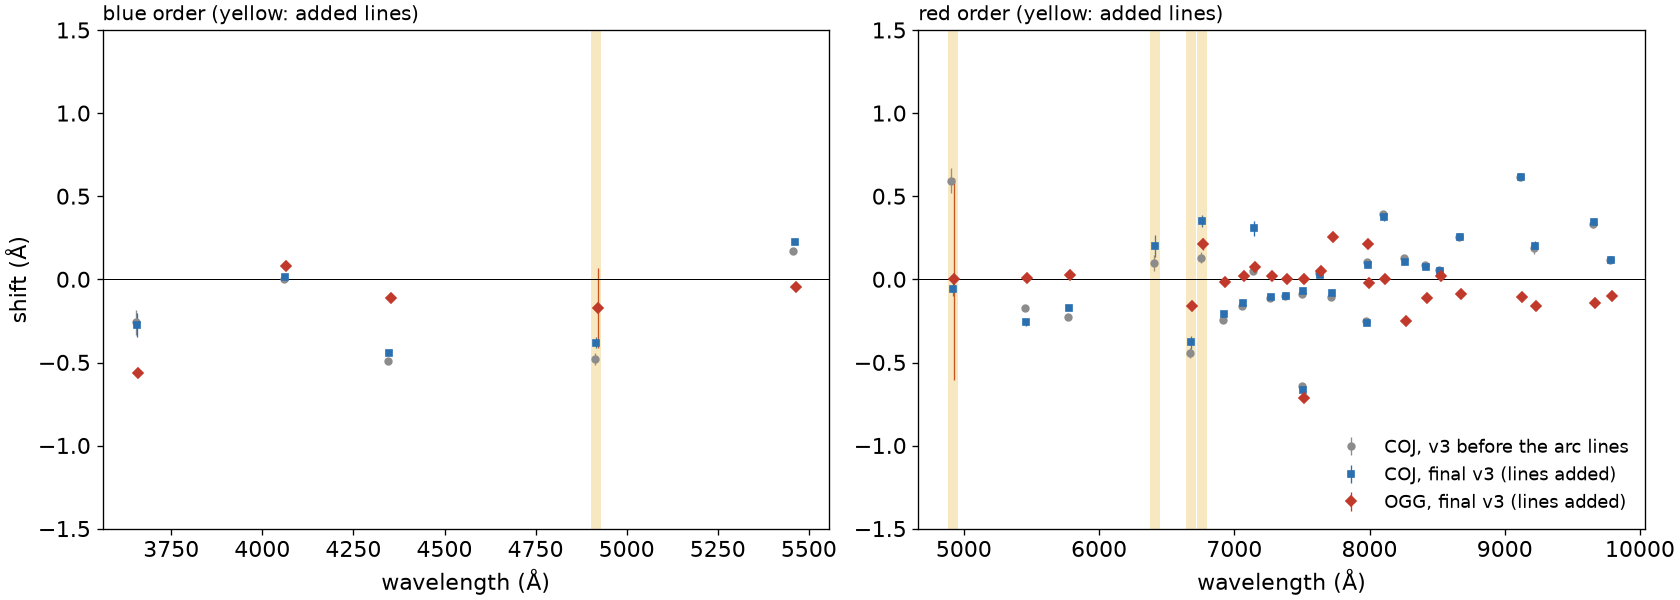
\includegraphics[width=\textwidth]{figures/fig_arc_lines.png}
\caption{Median shift of every arc line group on the arcs' own wavelength solutions (eq.~\ref{eq:arcgroup}), blue
order left and red right: COJ before (grey) and after (blue) adding the lines to the arc fit, and OGG with the lines
(red). Yellow: the added lines. Error bars: scatter over the arcs divided by $\sqrt{N}$.}
\label{fig:arc_lines}
\end{figure}

\section{A trace template for each site}
\label{sec:sites_trace}
The instrumental shape $S_o(\lambda)$ of the object-trace model (eq.~\ref{eq:tracemodel}) belongs to the instrument,
so OGG needs its own. It was built, as for COJ, from the chunk centroids of all OGG standards (100 frames; script
\texttt{build\_trace\_template.py}); it spans $-0.28$ to $+0.45$\,px (red) and $-0.17$ to $+0.21$\,px (blue), and the
smoothed template follows the stacked median to 0.014 and 0.012\,px. The priors are $c_1-c_2=-0.18\pm0.18$\,px and
$a=0.24\pm0.51$ (COJ: $-0.87\pm0.29$ and $0.58\pm0.14$). The fitted refraction scale varies much more from frame to
frame at OGG (the standards range from $\approx-0.1$ to 0.3, NGC\,4151 has $0.89\pm0.21$), so its prior is broad and
each frame's own centroids decide. Without a template the pipeline falls back to the 1.1.0 polynomial; with it, every
OGG frame uses the physical model (\texttt{L1TRCMOD = 'adr'}).

\section{Flux standards and a throughput step at OGG}
\label{sec:sites_flux}
In a first OGG reduction only BD$+28^\circ4211$ was a flux standard: GD\,153 and Feige\,67 are not in the \banzai{}
catalogue. NGC\,4151's [O\,{\sc iii}] flux, which should be constant, then scattered by 26 per cent, because of a
step: $6.8\times10^{-12}$ until 2025 March 28 and $1.2\times10^{-11}$\,erg\,s$^{-1}$\,cm$^{-2}$ from May 10, a factor of
1.8 in both orders. The step is real light: the raw counts and the sum over the whole order in 2-d show the same
factor, the extraction window holds 92--96 per cent of the light throughout, and the lamp flats and arcs (which do
not use the telescope) stay constant to 10 per cent. It is therefore a change of the telescope throughput between
2025 April 7 and May 2 (the last Feige\,67 and the first GD\,153 exposure): Feige\,67 in March--April comes out at
about half its catalogue flux, GD\,153 in May at its catalogue flux. All BD$+28^\circ4211$ standards are from after the
step (June--August), so every frame before it was calibrated $\approx1.8$ times too faint.

The fix is a standard before the step. Feige\,67 (Oke 1990, 3200--9200\,\AA; ESO \texttt{okestan}) and GD\,153 (ESO
X-shooter library) were added to \texttt{data/standards} in the format of the other references, at the positions LCO
observes them (GD\,153 is $5''$ from its J2000 position because of its proper motion). The Feige\,67 reference ends at
9200\,\AA, and the flux code holds a reference constant beyond its end, which would corrupt the red end of the
sensitivity; it is extended to 11\,000\,\AA{} with a power law fitted to its own 7500--9200\,\AA{} continuum (index
$-3.99$, the Rayleigh--Jeans slope of this hot subdwarf; header keywords \texttt{EXTRAP}, \texttt{EXTRAPSL}). With
the two standards, the NGC\,4151 [O\,{\sc iii}] flux scatters by 9.4 per cent (COJ Fairall~9: 12.5 per cent over all
100 spectra) and the levels before and after the step agree to 7 per cent (Fig.~\ref{fig:sites}); the remaining 7 per
cent is plausibly the older Feige\,67 reference against the HST-based ones. The scatter that remains at both sites
is mostly clouds and slit losses during the science exposures themselves (single exposures at 0.7 and 1.3 times the
median have low counts or high airmass), which no calibration can remove and which the RM scaling to
[O\,{\sc iii}] is designed for; the red/blue ratio, which they do not affect, scatters by 6--6.5 per cent. The 8 NGC\,4151 spectra of 2024 November and
December have no standard within 90\,d; they use the nearest one (Feige\,67, before the step) instead of an ensemble.

Two lessons follow. The ensemble of the nearest standards is only valid if the throughput does not change within it;
the nine nearest standards of a frame close to a step would mix both sides (here no NGC\,4151 frame falls between
April 7 and May 2, so this did not happen). And a campaign needs standards throughout, of a star in the catalogue
(Chapter~\ref{sec:recommendations}).

\section{The object zero point on NGC\,4151}
\label{sec:sites_zp}
NGC\,4151 is a strong test of the telluric zero point (Section~\ref{sec:wl_zp}): its zero points range from $-10$ to
$+17$\,\AA{} in the red order (median $+10.7$\,\AA), i.e.\ the nucleus sits up to $\approx\pm2''$ from the slit centre
from visit to visit. Before the correction the [O\,{\sc iii}] position scatters by 6.2\,\AA{} (red) and 3.1\,\AA{}
(blue); after it by 0.94 and 0.53\,\AA. Fairall~9 at COJ behaves the same way: without the correction its
[O\,{\sc iii}] position scatters by 6.5\,\AA{} (red) and 3.2\,\AA{} (blue) in the final reduction, with it by 0.69
and 0.45\,\AA{} (Fig.~\ref{fig:sites}). For both targets the correction is what aligns the epochs. Without this step the NGC\,4151
spectra would be misaligned by up to 27\,\AA{} between epochs.

\section{Verification of every step at both sites}
\label{sec:sites_verify}
Table~\ref{tab:sites} and Fig.~\ref{fig:sites} collect the measurements of every step, made with the same script on
both sites (\texttt{v3\_verify.py}). COJ is shown before and after the arc lines were added; the other COJ numbers
do not change. All 317 spectra use the physical trace model, the joint fringe and telluric fit, and (science frames)
the nine-standard telluric and flux ensembles.

\begin{table}[!htbp]
\centering
\caption{Verification of the final pipeline. Science: Fairall~9 at COJ (100 spectra), NGC\,4151 at OGG (60). Wavelengths
in \AA; residuals and scatters in per cent; pulls are the robust rms of $(f_1-f_2)/\sigma$ for the two exposures of
each visit (1 = correct uncertainties). Standards: rms of flux over reference in the clean windows (6500--7500\,\AA)
and at 7750--8900\,\AA.}
\label{tab:sites}
\small
\begin{tabular}{llccc}
\toprule
Step & Measurement & COJ, v3 before & COJ, final & OGG, final \\
 & & arc lines & v3 & v3 \\
\midrule
Arcs & median error of the used lines, rms (\AA) & 0.49 & 0.49 & 0.15 \\
 & largest median error at the added lines (\AA) & 0.59 & 0.38 & 1.3$^{a}$ \\
Trace & frames with the physical model (\%) & 100 & 100 & 100 \\
Zero point & science: [O\,{\sc iii}] scatter, red / blue (\AA) & 0.62 / 0.48 & 0.69 / 0.45 & 0.94 / 0.53 \\
 & science: [O\,{\sc iii}] red $-$ blue (\AA) & $+0.61\pm0.79$ & $+0.30\pm0.79$ & $+1.39\pm0.88$ \\
Fringes & science: red fringe metric (\%) & 2.01 & 1.95 & 2.51 \\
 & science: clean window 6960--7150\,\AA{} (\%) & 0.58 & 0.58 & 0.86 \\
 & science: same-visit difference, 6500--7500\,\AA{} (\%) & 0.65 & 0.66 & 0.69 \\
Telluric & science: water band 7170--7330\,\AA{} (\%) & 1.91 & 1.92 & 2.19 \\
 & science: water band 8130--8360\,\AA{} (\%) & 3.35 & 3.21 & 2.70 \\
Flux & science: [O\,{\sc iii}] flux scatter, blue / red (\%) & 12.6 / 13.3 & 12.5 / 14.0 & 9.4 / 12.5 \\
 & science: red/blue [O\,{\sc iii}] ratio scatter (\%) & 6.1 & 6.5 & 6.2 \\
 & standard over reference, 6500--7500 / 7750--8900\,\AA{} (\%) & 0.93 / 1.92 & 0.97 / 2.00 & 0.71 / 1.12$^{b}$ \\
 & independent star: EG\,21 shape, 6500--7500\,\AA{} (\%) & 1.13 & 1.09 & -- \\
Errors & science: pull, blue order (no unit) & 0.95--1.05 & 0.95--1.06 & 0.90--1.01 \\
 & science: pull, red order (no unit) & 0.93--1.07 & 0.94--1.06 & 0.98--1.27 \\
\bottomrule
\end{tabular}
\par\smallskip\raggedright\footnotesize
$^{a}$Ar\,6416, detected in only 3 OGG arcs. $^{b}$BD$+28^\circ4211$ (GD\,153: 1.16 / 2.23; Feige\,67: 0.90 / 1.47);
COJ: Feige\,110.
\end{table}

\begin{figure}[!htbp]
\centering
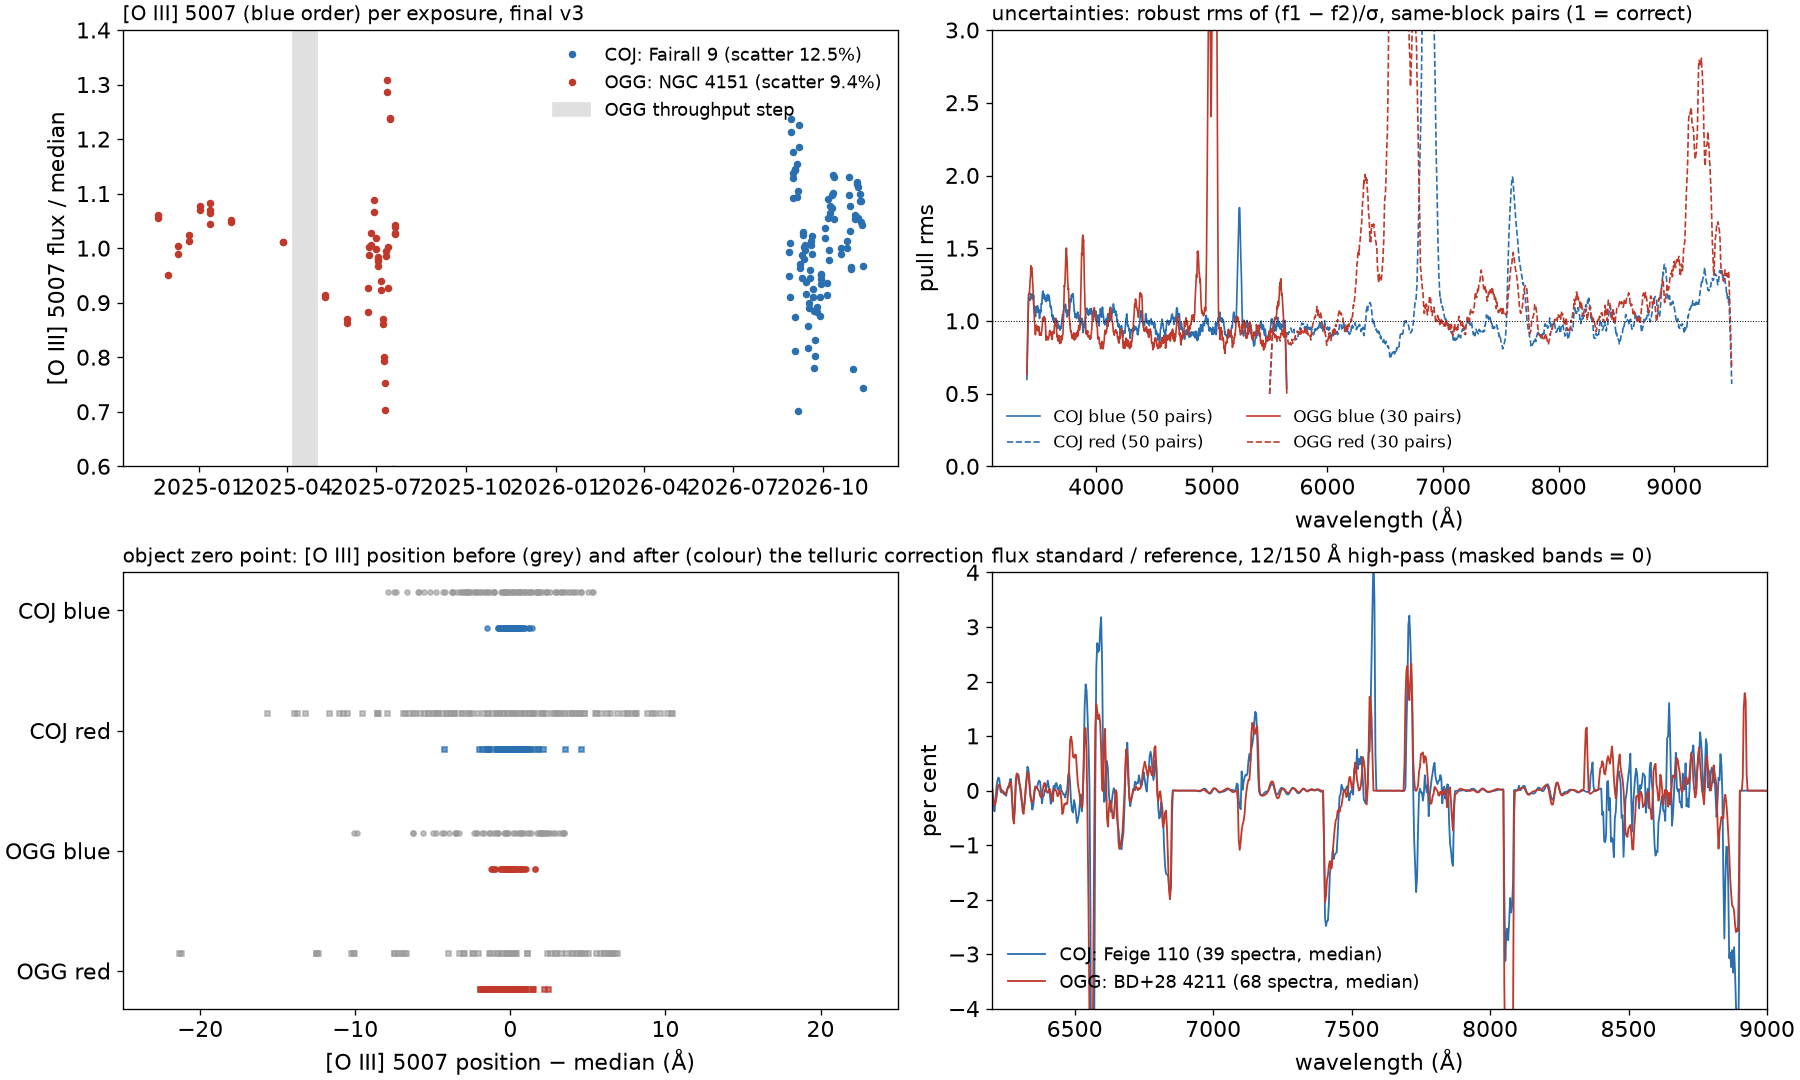
\includegraphics[width=\textwidth]{figures/fig_sites.png}
\caption{The final pipeline at both sites. Top left: [O\,{\sc iii}]\,5007 flux of every exposure (blue order) over
its median; grey band: the OGG throughput step, bridged by the added standards. Top right: pull rms of the two
exposures of each visit (1 = correct uncertainties). Bottom left: [O\,{\sc iii}] position of every exposure before
(grey) and after (colour) the telluric zero point. Bottom right: median flux standard over its reference at
fringe scales (Feige\,110 at COJ, BD$+28^\circ4211$ at OGG; the telluric bands are flat by construction).}
\label{fig:sites}
\end{figure}

\textit{Reading the comparison.} The two sites agree to within what their targets allow. The OGG pull rises to 1.2--1.3
redward of 6500\,\AA: NGC\,4151 has a 2.4 times higher signal-to-noise ratio per bin than Fairall~9, so the same fringe and telluric
residuals, which are not in the error array (Section~\ref{sec:raw_errors}), weigh more against the photon noise. The
red fringe metric of NGC\,4151 (2.5 per cent) includes its own O\,{\sc i}\,8446 and Ca\,{\sc ii}/Paschen lines in the windows; the
difference between the two exposures of a visit, which removes everything static, is the same at both sites
(0.66--0.69 per cent). The red--blue [O\,{\sc iii}] difference at OGG (1.4\,\AA) is larger than at COJ (0.3\,\AA)
because the added arc lines rarely enter the OGG fit; it is a constant per site and is removed by the usual alignment
on [O\,{\sc iii}].

\section{Disk space}
\label{sec:sites_disk}
A processed 2-d spectrum is 47\,MB, of which 43\,MB is the uncompressed \texttt{BINNED2D} table. None of the 2-d
diagnostic content is read back by the pipeline, so after a run the finished 2-d spectra are made lean
(\texttt{lean\_2d.py}: the \texttt{PROFILE}, \texttt{BACKGROUND} and \texttt{FRINGE} images are dropped, and
\texttt{BINNED2D} is kept only in a few example frames), and the arcs and lamp flats lose their \texttt{BINNED2D}
during the run. A site-season of $\approx$400 frames then takes $\approx2$\,GB, of which 1.2\,GB are the processed
calibrations kept for re-reducing the science; the \texttt{-1d} spectra are 0.6\,MB each.
